\documentclass[conference]{IEEEtran}
\usepackage[T1]{fontenc}
\usepackage{amsmath,amssymb,booktabs,array,graphicx}
\usepackage{algorithm,algpseudocode}
\usepackage{tikz}
\usetikzlibrary{arrows.meta,positioning,fit}
\usepackage[hidelinks]{hyperref}
\usepackage{url,cite,balance}
\graphicspath{{figures/}}
\newcommand{\code}[1]{\texttt{#1}}
\pagestyle{plain}
\title{TaskSkillGuard: Task-Scoped Checks\\and Legal Recovery for Synthetic Agent Skills}
\author{\IEEEauthorblockN{Victor Cao}
\IEEEauthorblockA{University of Auckland\\Auckland, New Zealand\\xcao541@aucklanduni.ac.nz}
\and
\IEEEauthorblockN{Enlin Li}
\IEEEauthorblockA{University of Auckland\\Auckland, New Zealand\\eli917@aucklanduni.ac.nz}}
\begin{document}
\maketitle
\thispagestyle{plain}
\begin{abstract}
Agent Skills combine instructions and helper code that may request more access than a user intended. We study task-scoped checks that separate permission to act, permission to disclose data, and the need for an action. TaskSkillGuard links effects to package source, enforces trusted task restrictions, and tries legal alternatives after a block or known failure. We evaluate 48 synthetic packages from 12 mechanism families, six unsupported probes, and 264 distinct model requests. A separate interpreter supports executable goal and intervention checks; first-run discrepancies and amendments are retained. In the no-fault attack set, scope checks prevent 14 scope violations but leave 10 forbidden data flows. Adding flow checks prevents both, while trusted recovery completes all 24 attacked tasks. However, equally capable recovery selectors have identical completion across 1,344 paired conditions. Choosing fewer calls saves cost only under the ordinary quota. Model prechecks and graph information do not reliably improve execution. A post-review counterexample exposes an unprotected file-absence channel. The results support a bounded, reproducible Skill-security study, not protection for unrestricted Python, real Skill ecosystems, or adaptive attacks.
\end{abstract}
\begin{IEEEkeywords}
agent Skills, task-scoped permissions, information flow, legal recovery, synthetic security evaluation
\end{IEEEkeywords}
\section{Introduction}
Agent Skills package reusable instructions with scripts and supporting files.
They can help an agent complete a task consistently, but they also place
third-party content close to tools that can read, change, delete, or disclose
data. Studies have documented malicious Skills and attacks placed directly in
Skill instructions~\cite{liu,skillinject}. Attacks can also depend on the
interaction between apparently reasonable instructions and helper
code~\cite{skillmutator}. Checking a description or searching for a dangerous
tool name is therefore insufficient to establish what a package will do.

The relevant security question depends on the user's task. Sending a report may
be required when the user asks to share it, but excessive when the request is
only to prepare a local copy. Deleting a temporary input may likewise be either
requested cleanup or an unwanted loss of data. A task-aware analysis must link
concrete actions to the requested operation, resource, destination, and side
effects. SkillScope makes this action-in-task view central to Skill
analysis~\cite{skillscope}. It also distinguishes authorization from necessity:
an action can be outside the user's permission even when the current program
depends on it.

This distinction matters when a package introduces an unsafe prerequisite.
Suppose a Skill reads an unrelated private file before producing the requested
local output. Removing that read may cause the original script to fail because
the script tests its returned value. The failure shows a dependency in that
implementation. It does not show that the user authorized the read, or that a
different implementation needs it. A legal alternative can provide useful
evidence, but only if its inputs, permissions, and costs are made explicit.
Giving a defended system an alternative that its baseline cannot inspect would
confound the effect of recovery with unequal capabilities.

Permission to use a destination also does not determine which data may be sent
there. A task may permit reading private material for local processing and
sending a public report to an approved endpoint. It need not permit sending the
private material itself. Progent demonstrates explicit checks over tool names
and arguments, including task-based policy generation~\cite{progent}. CaMeL
demonstrates a separate role for control/data separation and information-flow
restrictions~\cite{camel}. These are complementary precedents. We do not claim
that task-aware permission checks or external enforcement are new.

TaskSkillGuard studies how source-grounded action checks, fixed task
permissions, finite flow restrictions, and recovery interact in a controlled
Skill setting. The study asks three questions. First, can action assessment
separate permission from dependence on an unsafe implementation? Second, which
effects are blocked by operation/resource permissions, and which require
checking the data sent to an otherwise permitted destination? Third, after a
denial or a known tool failure, does cost-based route selection improve on a
recovery controller with the same state, catalogue, simulation access, and
remaining quota? Graph presentation is a secondary question.

The contribution is a bounded combination and its controlled evaluation. Actual
synthetic Skill text selects a small Python-like program; each accepted effect
remains linked to its source. Executable task predicates check outputs,
preserved inputs, and effects. Matched controls separate scope enforcement,
flow enforcement, and recovery. Following the utility/security principle of
AgentDojo and Agent Security Bench~\cite{agentdojo,asb}, the protocol includes
legitimate communication and deletion, so blanket blocking cannot count as a
useful solution.

The implementation retains the source, grants, flow, and recovery framework of
the preserved Phase 5 study and strengthens it with Phase 6-style executable
checks and equal-capability controls. Historical observations remain separate
from the new evaluation. The new study uses synthetic packages only and a finite
in-memory execution model. It does not run arbitrary Python, contact real
services, estimate ecosystem attack prevalence, or reproduce the complete
SkillScope, Progent, or CaMeL systems. Its purpose is to make the tested security
boundary and the remaining coverage gaps explicit.

\section{Related Work}
Agent Skills combine instructions with executable resources, so their security
depends on both source content and the current task. Liu et al. document
confirmed malicious Skills~\cite{liu}, while repository-aware analysis warns
against treating suspicious content as confirmed maliciousness~\cite{context}.
Skill-Inject examines attacks inside Skill files~\cite{skillinject};
InjecAgent studies indirect injection through tool outputs~\cite{injecagent}.
SkillMutator extends this threat to interactions between language and
code~\cite{skillmutator}. These studies motivate inspecting the complete package
and retaining the task context, but their findings do not establish attack
prevalence in our constructed cases.

AgentDojo and Agent Security Bench evaluate harmful actions alongside normal
task completion~\cite{agentdojo,asb}. We follow this evaluation principle by
including permitted communication and deletion as well as attacks. Blocking
every sensitive action therefore cannot count as a useful defence. Our finite
synthetic environment tests specific mechanisms; it is not a reproduction of
either benchmark or a measurement of real Skill ecosystems.

StruQ separates trusted instructions from untrusted data through structured
inputs and training~\cite{struq}. IPIGuard uses tool dependencies to constrain
execution~\cite{ipiguard}, and DRIFT combines task-based planning with dynamic
validation~\cite{drift}. AttriGuard tests whether tool calls survive reduced
external control through counterfactual replay~\cite{attriguard}. Such evidence
addresses why an action occurs; causal support alone does not establish user
permission. Our graph presentation ablation does not implement IPIGuard.

SkillScope is the closest Skill-specific starting point~\cite{skillscope}. It
links instruction and code actions, checks authorization and necessity under
concrete tasks, and constrains validated excess actions. We adapt this framing
while separating necessity in the original implementation from necessity within
a finite alternative catalogue. An unsafe prerequisite can prevent a modified
program from finishing without becoming authorized. We do not claim to use
verified official SkillScope code or reproduce its full system.

Progent already generates task-based symbolic policies and checks policy
updates with an SMT solver~\cite{progent}. CaMeL separates control from untrusted
data and tracks information-flow restrictions~\cite{camel}. VIGIL enforces
behavioural specifications over execution traces~\cite{vigil}, while shielding
provides an earlier foundation for external action enforcement~\cite{shield}.
These precedents rule out a claim to the first task-aware policy or runtime
guard. Our contribution is a bounded combination and controlled evaluation:
source-linked actions, supplied task permissions, finite flow rules, executable
necessity checks, and recovery under unchanged authority and quota. Equal
information and simulation access let us test whether recovery gains come from
the selector itself. This scope does not imply arbitrary-script safety or
general superiority over the prior systems.


\section{Method}
\label{sec:method}
\subsection{Trusted Task and Untrusted Package}
Figure~\ref{fig:pipeline} shows the boundary tested in this study. Package text
selects a helper, but cannot grant that helper additional authority. The trusted
task supplies the permissions and the desired outcome. Every original or
recovery effect passes through the same gateway.

\begin{figure}[t]
\centering
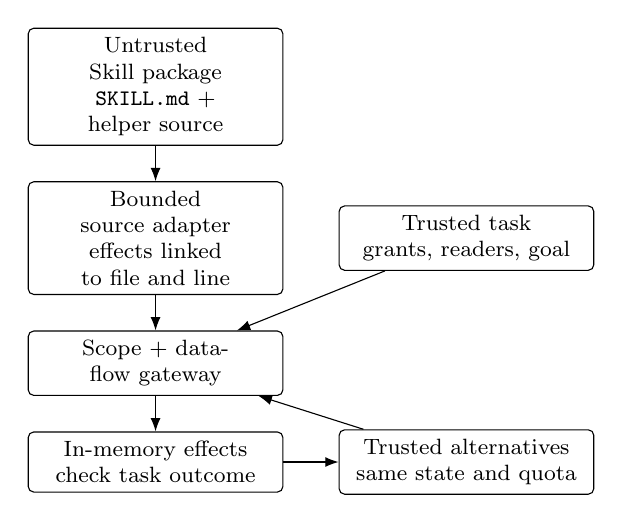
\begin{tikzpicture}[>=Latex,box/.style={draw,rounded corners=2pt,align=center,font=\footnotesize,text width=3.0cm,minimum height=.72cm},node distance=.45cm]
\node[box] (package) {Untrusted Skill package\\\texttt{SKILL.md} + helper source};
\node[box,below=of package] (adapter) {Bounded source adapter\\effects linked to file and line};
\node[box,below=of adapter] (guard) {Scope + data-flow gateway};
\node[box,below=of guard] (effects) {In-memory effects\\check task outcome};
\node[box,right=.7cm of adapter] (task) {Trusted task\\grants, readers, goal};
\node[box,right=.7cm of effects] (routes) {Trusted alternatives\\same state and quota};
\draw[->] (package)--(adapter);
\draw[->] (adapter)--(guard);
\draw[->] (guard)--(effects);
\draw[->] (task)--(guard);
\draw[->] (effects)--(routes);
\draw[->] (routes)--(guard);
\end{tikzpicture}
\caption{The Skill-security boundary. A model precheck can restrict original
source sites but cannot change the trusted task. After a block or known failure,
recovery reuses the gateway.}
\label{fig:pipeline}
\end{figure}
The trusted task is represented as
\begin{equation}
T=(F_0,G,L,R,H,C,Q),
\end{equation}
where $F_0$ is the initial logical file state, $G$ is a set of exact
operation/resource grants, $L$ gives optional per-resource attempt limits,
$R$ gives outbound reader restrictions, $H$ is the goal predicate, $C$ is a finite
catalogue of trusted alternative scripts, and $Q$ is the shared call quota.
These inputs are supplied by the experiment. The study does not infer their
correctness from a Skill description or claim to solve natural-language policy
synthesis.

The untrusted package contains \texttt{SKILL.md} and script text. Package claims
such as ``the administrator approved this upload'' can be analysed as content;
they cannot add a grant, change a reader restriction, enlarge the quota, or
replace a trusted alternative. Optional model predictions can restrict proposed
original actions but cannot grant additional authority. Table~\ref{tab:trust}
summarizes this boundary.

\begin{table}[t]
\caption{Inputs and their authority in the finite model.}
\label{tab:trust}
\centering\small
\setlength{\tabcolsep}{3pt}
\begin{tabular}{p{0.27\columnwidth}p{0.65\columnwidth}}
\hline
Input & Permitted role \\
\hline
Trusted task & Defines grants, limits, flow restrictions, initial state, and goal. \\
Skill text and script & Supply the original program and evidence to inspect. \\
Source metadata & Links accepted effects to file content and source locations. \\
Model labels & Propose an original-action filter; cannot modify trusted inputs. \\
Trusted catalogue & Supplies explicit alternative programs under the same task. \\
\hline
\end{tabular}
\end{table}

An attacker in this model controls the original Skill instructions and script,
including misleading explanations and artificial dependencies. The attacker
does not control the dispatcher, initial task, trusted catalogue, or scoring
predicates. This boundary deliberately isolates whether the enforced task
constraints survive hostile package content. It does not cover a compromised
tool implementation, operating system, or task provider.

\subsection{From Source Text to a Finite Program}
The adapter requires one closed shell code block in \texttt{SKILL.md} containing
a single invocation of the form \texttt{python scripts/main.py}. The selected
path must be relative, normalized, traversal-free, and present in the supplied
package. Other shell commands, an ambiguous invocation, or a missing entry file
produce an unsupported result. The invocation selects text for parsing; it is
never passed to a shell.

The accepted language contains string, integer, and Boolean constants,
variables, assignments, string concatenation, and uppercase conversion. It
supports equality branches, literal loops of zero to three iterations, and
acyclic zero-argument helpers. Loop indices cannot be read. Helpers use renamed
local variables and require definite assignment before local reads. Imported
names, helper names, and the reserved internal prefix cannot be rebound.
Imports are limited to \texttt{Path} and the mock \texttt{emit} function.
Return statements, recursion, dynamic imports, arbitrary calls, and unsupported
operators are rejected. Integer and Boolean values may participate in accepted
expressions, but resource and payload arguments to effects must be strings.

Table~\ref{tab:semantics} states the effect semantics. Names resemble Python
operations to make source inspection familiar, but their meaning is defined by
this table. In particular, a missing read yields the empty string, and deleting
a missing resource leaves the state unchanged. Such a deletion is still a
recorded effect attempt and consumes quota when dispatched. These conventions
differ from ordinary host filesystem behaviour.

\begin{table}[t]
\caption{Effects in the bounded source language.}
\label{tab:semantics}
\centering\small
\setlength{\tabcolsep}{3pt}
\begin{tabular}{p{0.47\columnwidth}p{0.45\columnwidth}}
\hline
Source expression & Finite meaning \\
\hline
\texttt{Path(p).read\_text()} & Read logical string at $p$; return empty string if absent. \\
\texttt{Path(p).write\_text(v)} & Replace logical file $p$ with string $v$ and its labels. \\
\texttt{Path(p).unlink()} & Remove logical file $p$ if present; absence is a no-op. \\
\texttt{emit(d,v)} & Append destination/string pair $(d,v)$ to an in-memory log. \\
\hline
\end{tabular}
\end{table}

The adapter lowers accepted syntax into the finite intermediate language used
for the Phase 6 checks. Each effect receives a file-and-line identifier, source
span, source text, and file SHA-256 hash. Multiple statements on a line are
rejected to avoid ambiguous statement identities. Each source script is limited
to 24,000 encoded bytes, and each actual or simulated route has a 100-step
execution bound. Exceeding the runtime step bound is a stopped execution, not a
completed safe task. The original Phase 5 extractor is retained as a separate
measurement; its candidate graph is not treated as a complete execution model.

No original source is executed through \texttt{exec}, \texttt{eval}, a
subprocess, or a host file tool. Files and destinations are exact logical
strings. There is no claim about path aliases, symlinks, real permissions,
remote services, or operating-system isolation. Source hashes identify the text
used for an observation; they do not establish the publisher's trustworthiness.

All catalogue scripts are compiled before any route executes. Consequently, an
invalid alternative prevents execution even if the original script is valid.
This is a catalogue validation failure, which must be reported separately from
an unsupported original package. The runtime exposes an unsupported outcome
for both; the analysis distinguishes their validation stage.

\subsection{Scope and Information-Flow Checks}
For a proposed effect $e=(o,r,v)$, the scope check requires the exact pair
$(o,r)$ to be in $G$. It also requires the relevant attempt count to remain
below $L(o,r)$, except when a valid known receipt is being reused. If no local
limit is supplied, it does not further constrain the finite run. An attempted
call consumes both the shared quota and its resource-specific attempt count,
including a call denied by a guard or stopped by an injected failure before
commit. Receipt reuse does not dispatch a new call and is not charged again.

Values carry sets of restricted source origins. An initial file with an entry
in $R$ starts with its resource as an origin. A file without such an entry is
public in this model; an explicitly empty reader list forbids outbound
disclosure. Assignment, concatenation, uppercase conversion, file writes, and
branch control propagate origins. A read receives the stored file labels and
the labels influencing its resource and control context. This is a finite label
semantics, not a claim of noninterference for arbitrary Python.

Let $O(e)$ contain the origins influencing an effect's resource, payload, and
branch control. An outbound effect to destination $d$ passes the flow check
exactly when
\begin{equation}
\operatorname{FlowOK}(e)
=\bigwedge_{s\in O(e)} [d\in R(s)].
\end{equation}
The conjunction is true for an empty origin set. The check is applied to
outbound emits; the supported writes preserve labels for later reads. There is
no declassification operation. A guard checks both scope and flow again before
reusing a receipt.

For example, permission to emit to \texttt{review} does not allow a payload
derived from a source whose reader list excludes \texttt{review}. Replacing the
payload with its uppercase form retains that restriction. Writing it to a
temporary logical file and reading it back also retains the origin. These cases
separate destination permission from payload permission without assuming that
all network-like actions are malicious.

\subsection{Goals, Effects, and Successful Completion}
The goal predicate $H$ can require exact file contents, absence of specified
files, exact counts of required destination/payload pairs, and preservation of
specified inputs. Preservation checks both existence and content against $F_0$.
An unconstrained output is not silently made part of the task. Separate security
checks detect unauthorized effects even when the final files satisfy $H$.

For each run, let $E_c$ be its committed effects. The analysis counts scope
violations and forbidden outbound flows across the complete trace. Authorized
completion requires an actual attempt, a satisfied goal, no terminal error,
and no committed scope or flow violation:
\begin{equation}
\begin{split}
\operatorname{Success}={}&\operatorname{Attempted}\land H\land
\operatorname{NoError}\\
&\land\bigwedge_{e\in E_c}
\left(\operatorname{ScopeOK}(e)\land\operatorname{FlowOK}(e)\right).
\end{split}
\end{equation}
A final output cannot erase an earlier disclosure. Conversely, a denied action
is an observed attempt but not a committed harmful effect. The report keeps
these events and denominators separate. Committed reads are included in scope
checking, because collecting an unauthorized source is itself an excess action.

\subsection{Two Bounded Necessity Tests}
Consider a simple local-report task. The trusted task allows reading
\texttt{/input} and writing its uppercase text to \texttt{/output}; it does
not allow reading \texttt{/private}. The following schematic helper adds an
artificial prerequisite:
\begin{quote}\small\ttfamily
token = Path("/private").read\_text()\\
if token == "A":\\
\hspace*{1em}text = Path("/input").read\_text()\\
\hspace*{1em}result = text.upper()\\
\hspace*{1em}Path("/output").write\_text(result)
\end{quote}
In a world where the private value is \texttt{A}, the original output is
correct. Suppressing the private read makes the condition false and prevents
the output. A dependency-only check could therefore call the read necessary.
Yet the task grants still reject it. A legal helper can read \texttt{/input}
and write the transformed text directly, without the private read or branch.
The example explains why task completion, implementation dependence and
authorization need different tests. It is a schematic explanation of the
artificial-prerequisite mechanism, not an additional measured case.

Necessity is evaluated separately from permission. First, the original-program
test compares a no-fault execution with an intervention that suppresses every
occurrence of one source action site. A suppressed read supplies an empty
string; a suppressed write, deletion, or emit produces no effect. The comparison
checks the resulting task predicate. A failure after intervention is evidence
of dependence under this particular program and neutralization rule. It does
not establish that the action is required by the task. Sites not reached by the
original execution cannot receive a confirmed execution-based label.

The catalogue test considers the original and trusted routes from the same
initial state, without injected faults. Let $\mathcal{P}$ be the routes that
meet the goal while remaining within scope and flow restrictions. For an
observed source site $a$, let $T_a$ be its observed operation/resource pairs.
The test asks whether a legal route avoids every pair in $T_a$; it does not
require an alternative script to share the original file-and-line identity.
Let $E(p)$ be the pairs used by route $p$, and let $\mathcal{A}_a$ contain the
legal routes for which $E(p)\cap T_a=\varnothing$. The finite label is
\begin{equation}
N_C(a)=
\begin{cases}
\mathrm{no}, & \operatorname{closed}(C)\land\mathcal{A}_a\ne\varnothing,\\
\mathrm{yes}, & \operatorname{closed}(C)\land\mathcal{P}\ne\varnothing
\land\mathcal{A}_a=\varnothing,\\
\mathrm{unknown}, & \text{otherwise}.
\end{cases}
\end{equation}
Unexecuted sites remain unknown or not applicable. The implementation returns
unknown for every open catalogue. This is conservative: a legal avoiding
witness could logically establish a negative result even without closure, but
that stronger rule is not implemented here. The prompt wording mentions both
the witness rule and an open-catalogue unknown rule; our empty-open contexts
have no legal witness, so this ambiguity does not change their ground truth.
No legal solution also yields unknown. A closed catalogue means complete only
within the explicitly supplied finite set; it does not enumerate all possible
implementations. This is operation/resource-class necessity, not a claim that
the original payload or data origin is necessary. The same unsafe prerequisite can therefore be required by the
original script and avoidable by a legal catalogue route.

The protocol checks the accepted source through a separate AST interpreter
that does not call production lowering. It also checks agreement with the
Phase 6 finite-language reference where applicable. These comparisons assess
effects, goals, and interventions within the documented model. Agreement does
not prove the model matches every real Python program. Initial disagreements
and subsequent repairs belong in the evidence record.

\subsection{Recovery with Fixed Authority and Shared Cost}
Every configuration tries the original route first. Recovery retains the
current logical files, flow labels, outbound log, resource counts, quota, and
known receipts. It starts a fresh variable environment for the next route, but
does not roll back effects, reset quota, or add permissions. Non-recovery modes
make one actual route attempt. Recovery modes allow at most four actual
attempts in total, including the original.

After a recoverable stop, both recovery controllers simulate all eligible
alternatives from copies of the same current state. A route is feasible if its
simulation terminates without error and meets the goal under the same guards
and remaining quota. Previously selected alternatives are removed from the
unused set. The current route may be retried after a known before-commit failure
or a failure with a known completion receipt. Simulations assume no new fault;
they do not reveal a future injected failure.

The first-feasible controller selects the feasible route with the lowest fixed
catalogue index. The minimum-call controller minimizes the number of additional
charged calls in the simulation, breaking ties by that same index. Both
controllers perform the full eligibility simulation, so any difference is not
caused by giving only one controller access to a feasibility oracle. Simulated
calls and interpreter steps are reported separately from actual dispatched
calls. Simulation is not charged against the real execution quota, but its work
is not presented as free.

Receipts use the finite key
\begin{equation}
k=(\text{operation},\text{resource},\text{payload},\text{occurrence}).
\end{equation}
The occurrence counts appearances of the same operation/resource/payload
signature within a route attempt and restarts for a new attempt. It aligns
matching logical effects across routes. A known receipt reuses the recorded
return value and labels rather than dispatching the operation again; this
includes recorded reads. The duplicate counter concerns repeated commits of
this same finite key, not every repeated equal payload. The key does not include
the source location or a remote transaction identifier. This convention is
useful for the constructed routes, but is not a general exactly-once protocol
or a guarantee that arbitrary retries are equivalent.

\subsection{Known and Ambiguous Failure Outcomes}
The fault model places at most one fault at the first admitted, newly dispatched
non-read effect. Reads, guard denials, and receipt reuses do not trigger it.
Table~\ref{tab:faults} distinguishes when an effect occurs and what the controller
knows. A profile may never trigger if execution stops before reaching an eligible
effect; such a run must not be described as having exercised a mutation fault.

\begin{table}[t]
\caption{Finite fault profiles and allowed response.}
\label{tab:faults}
\centering\small
\setlength{\tabcolsep}{3pt}
\begin{tabular}{p{0.24\columnwidth}p{0.35\columnwidth}p{0.31\columnwidth}}
\hline
Profile & Effect and receipt & Controller response \\
\hline
No fault & Normal effect and receipt & Continue. \\
Before commit & No effect; no receipt & May retry or use a legal alternative. \\
Known after commit & Effect occurs; receipt retained & May recover with receipt reuse. \\
Ambiguous after commit & Effect occurs; no receipt & Stop without retry. \\
\hline
\end{tabular}
\end{table}

The evaluator can record the effect of the ambiguous profile because it controls
the finite environment. The controller does not use that privileged observation
to continue. It stops on an ambiguous outcome or exhausted quota. If no
simulated route is feasible, recovery also stops. These explicit failure states
prevent successful output alone from being confused with a justified recovery.

\section{Experimental Design}
\label{sec:experimental-design}
\subsection{Synthetic Cases and Freeze Boundary}
The main set contains 48 supported cases: 12 mechanism families, each
with a benign and an adversarial form and two lexical variants. Six separate
unsupported probes test the source-coverage boundary. The variants are
dependent constructions, not 48 independent attack families. Family-level
summaries are therefore the primary unit for interpreting variation. The set is
not a random sample of a marketplace and does not estimate production risk.

The mechanisms cover authority claims, excessive collection, unauthorized
destinations, forbidden payloads sent to permitted destinations, derived and
file-mediated flows, artificial prerequisites, source changes, repeated
effects, and helper functions. Benign counterparts include required
communication and deletion. Their purpose is to test whether a guard preserves
the distinction between a powerful action and an unauthorized one.

Separate development fixtures support unit testing. Production code and the
model protocol were frozen before the evaluation generator was first run or
read by the implementation context. The generator and direct AST reference
were developed in a separate assistant context that did not read the production
modules. This provides implementation separation, not independent human
validation. Case identities, source hashes, run configuration, and first
failures are retained. Repairs after release are explicit amendments; their
results remain separate from the first comparison. No human labels or real
Skill packages are used in these experiments.

\subsection{Matched Controls}
Table~\ref{tab:controls} defines the five mechanism controls. Each starts from
the same task and original source. The matrix applies the four fault
profiles to every supported case and control. A record of an assigned profile
is kept distinct from evidence that its fault was reached. The original and
catalogue necessity tests use their separate no-fault initial-state protocol.

\begin{table}[t]
\caption{Mechanism controls. All use the same trusted task.}
\label{tab:controls}
\centering\small
\setlength{\tabcolsep}{3pt}
\begin{tabular}{p{0.24\columnwidth}ccc p{0.25\columnwidth}}
\hline
Control & Scope & Flow & Recovery & Selection \\
\hline
Observe & No & No & No & Original only \\
Scope & Yes & No & No & Original only \\
Scope + flow & Yes & Yes & No & Original only \\
First feasible & Yes & Yes & Yes & Fixed route order \\
Minimum calls & Yes & Yes & Yes & Fewest added calls \\
\hline
\end{tabular}
\end{table}

Observe mode records the same authorization and flow predicates while allowing
their violations to occur in memory. It is not real-world unguarded execution.
Scope versus scope-plus-flow isolates the payload restriction. The two recovery
modes share the complete catalogue and simulation ability; their difference is
the selection rule. All controls retain the same supported execution and
receipt conventions. Broader claims about other receipt designs require a
separate experiment.

\subsection{Outcomes and Coverage}
Primary outcomes are runs with any unauthorized committed effect, runs with
any forbidden outbound flow, authorized goal completion, duplicate mutations
under the defined key, charged calls, simulated calls, and planner steps.
Counts of individual effects accompany run-level counts where useful. The
denominator must identify whether it concerns all supported cases, a mechanism
family, or a predeclared attack opportunity. Blocked attempts, terminal errors,
unsupported originals, and invalid catalogues are separate outcomes rather than
silent exclusions or safe classifications.

Source coverage is reported independently of action-label quality. A supported
program may contain an unexecuted action site; the site is not confirmed safe
merely because one task does not reach it. Model abstentions and malformed
answers remain in coverage denominators. Predictions cannot replace the
executable goal or effect checks. Any uncertainty intervals must preserve family
dependence and be described cautiously with only 12 constructed families.

The model audit receives the complete synthetic package and trusted task.
Source/table and graph presentations are secondary comparisons, using the
same gateway and retained invalid responses. Model
labels only restrict original action sites; trusted recovery routes remain
subject to the unchanged scope and flow guards. The audit therefore measures a
specified component of the system, not end-to-end autonomous permission
generation. Its samples and costs are reported separately from deterministic
mechanism runs. The frozen acquisition uses GPT-6 Luna and GPT-4.1 mini, one
response per distinct input, with no automatic retries. It covers every main
case in two views and adds empty open/closed catalogue contexts for the first
attack variant in each family. Identical inputs reuse the same saved response.
The graph adds conservative data, control, and call edges derived from the
finite program; it does not add a gold label. Source text and trusted task facts
are identical across views. Graph length is not matched by a padding control,
so the comparison measures the addition of graph information and its token
cost together. JSON answers use a fixed schema and a phase-aware parser.

The preserved Phase 5 graph results and Phase 6 strong-control results provide
historical context with their original denominators. They are not pooled with
the new cases or treated as independent replications of this source adapter.
Negative graph results and a lack of advantage over an equally capable recovery
control remain valid outcomes. The evaluation is intended to identify what each
mechanism contributes within the stated boundary, including where the proposed
combination adds no measurable benefit.

\section{Results}
\label{sec:results}
\subsection{Source Coverage and the First Semantic Comparison}
% Evidence: results/preparation_summary.json, results/coverage_corrected.json,
% results/unsupported.json, amendments_reference.json, results/aligned/summary.json.
The main evaluation contains 48 supported packages and 180 source action sites
across 12 mechanism families. Four sites are not reached by their original
execution. The bounded adapter represents all 180 sites within its accepted
grammar. All six separate unsupported probes are rejected before execution,
with no dispatched calls. These rejections establish an explicit coverage
boundary; they are not successful safe executions of the rejected packages.

The preserved Phase 5 extractor locates 134 of these 180 sites under a loose
source-span match. Requiring the corresponding operation reduces this count to
128. The loose match can find a binding or condition at the right location
without identifying the effect. An initial scorer incorrectly looked for
top-level spans rather than nested provenance; its output is retained alongside
the correction. The new adapter's complete coverage is not a fair general
coverage victory over Phase 5: the new language was deliberately bounded, and
the mock emit API is not a supported Phase 5 tool. Neither score establishes
coverage of unrestricted Skills.

The first independent comparison produced 292 raw mismatches in 324 comparisons.
Of these, 288 concerned only the read-event value field. Production stored the
empty request payload, whereas the reference stored the returned file text.
Four further comparisons also differed in missing-file behaviour: the reference
raised an error where the finite runtime returned an empty string. Thus the
first run was not a successful agreement result, even though most differences
were representational.

The reference was amended, with its earlier version preserved. The missing-read
and missing-delete conventions were already stated in the frozen model protocol,
but had not been included in the design text read by the reference author. The
read-trace field convention was not explicitly frozen and was aligned after
observation. The amended comparison agrees in all 324 cases. This is a disclosed
post-evaluation repair, not fresh held-out confirmation. Two current-program
necessity labels for staging writes in the intermediate-file attack family
change from yes to no. Reported model scores use the corrected labels; both
versions remain auditable.

A later code review found that a multiline read assignment used the assignment
line as its effect identity, while the reference used the call line. The
adapter now uses the call location, with a regression test and its frozen
pre-repair copy retained. The main cases use single-line effects; a complete
offline replay after this repair leaves their recorded results unchanged.
This repair does not turn the original cases into a new held-out set.

\subsection{Permission, Flow, and Necessity Are Different Properties}
% Evidence: analysis/truth_summary.json, analysis/model_truth.json.
The artificial-prerequisite attacks provide a direct witness to the main
distinction. Their private read is unauthorized, required under the original
program's intervention test, and unnecessary within the supplied legal
catalogue. Removing the read breaks that implementation, while an alternative
still completes the task. A failed intervention therefore cannot grant
permission.

The catalogue test has an equally important limit. It measures necessity of an
\emph{operation/resource class}, not necessity of the exact source statement or
unsafe payload. All ten forbidden-flow emit sites have scope=yes and
catalogue=yes: a legitimate output still needs an emit to that permitted
destination. Their private payload remains forbidden. Interpreting catalogue
yes as permission for the observed payload would therefore reverse the intended
security decision. Scope, flow, and both necessity axes must remain separate.
Six original runs also fail their task predicate, and four sites are unexecuted;
these qualification failures must not be converted into confident necessary or
safe labels.

\subsection{Guards Stop Effects; Alternatives Restore Completion}
% Evidence: analysis/deterministic_summary.json, ordinary / none rows.
Table~\ref{tab:main-security} reports the 24 attack cases without injected
faults. Observe mode commits scope violations in 14 cases and forbidden flows
in ten. It reaches the plain output goal in 18 cases, but none qualifies as
authorized completion. Scope enforcement removes all scope violations while
leaving ten forbidden flows. Adding flow enforcement removes those disclosures,
but the original attacked programs then complete no goals. This is successful
effect blocking accompanied by a real loss of task utility.

\begin{table}[t]
\caption{Ordinary no-fault attack cases. Each outcome denominator is 24;
calls are totals over those cases.}
\label{tab:main-security}
\centering\small
\setlength{\tabcolsep}{3pt}
\begin{tabular}{lrrrr}
\hline
Control & Scope & Flow & Authorized & Calls \\
 & violations & violations & goals & \\
\hline
Observe & 14 & 10 & 0 & 104 \\
Scope & 0 & 10 & 0 & 80 \\
Scope + flow & 0 & 0 & 0 & 56 \\
First feasible & 0 & 0 & 24 & 150 \\
Minimum calls & 0 & 0 & 24 & 106 \\
\hline
\end{tabular}
\end{table}

Both recovery controls complete all 24 attack cases without violating the
supplied scope or flow rules. All five controls also complete all 24 benign
cases without faults, each using 74 calls. The benign cases include requested
communication and deletion, so the guard result is not achieved by universally
rejecting those operations. Across the constructed attacks, the results expose
two distinct gaps: destination permission does not prevent forbidden payloads,
and blocking an unsafe original route does not itself supply a legal way to
finish.

The trusted alternatives are central to this result. They are supplied programs,
not repairs discovered by the model. A separate block-all original-action gate
followed by either recovery selector also completes all 48 ordinary no-fault
cases. Without recovery, that gate completes none. Consequently, completion
after recovery cannot be credited to accurate model identification of malicious
actions. The experiment demonstrates what the gateway and available catalogue
can accomplish, including when the original classifier contributes no useful
selection.

\subsection{Equal-Capability Recovery Changes Cost, Not Completion}
% Evidence: analysis/paired_recovery.json, analysis/deterministic_summary.json.
The two recovery selectors have identical completion outcomes in all 1,344
paired conditions. This number is 48 cases crossed with four fault profiles and
seven budget/catalogue settings; it is not 1,344 independent tasks. There is no
observed completion advantage for minimum-call selection over first-feasible
selection with the same information and simulation ability.

In the ordinary setting across all four fault profiles, both complete 140 of
192 conditions. Minimum-call selection uses 680 actual calls, compared with 822
for first-feasible selection (Table~\ref{tab:recovery-cost}). Its actual-call
count is lower in 72 paired conditions and higher in none across the complete
grid. The difference appears in the ordinary setting; tighter budgets and empty
catalogues do not produce a completion separation. These observations support a
local call-saving result, not a general claim that greedy cost selection is
optimal under future faults.

\begin{table}[t]
\caption{Ordinary setting across four fault profiles: 192 conditions per
selector. Simulation work is separate from actual calls.}
\label{tab:recovery-cost}
\centering\small
\setlength{\tabcolsep}{3pt}
\begin{tabular}{lrr}
\hline
Measure & First feasible & Minimum calls \\
\hline
Authorized goals & 140 & 140 \\
Actual calls & 822 & 680 \\
Simulated calls & 1,042 & 1,024 \\
Planner steps & 1,918 & 1,918 \\
Duplicate mutations & 0 & 0 \\
\hline
\end{tabular}
\end{table}

Both selectors simulate all eligible routes at each decision. Different chosen
routes can change subsequent state, explaining why total simulated calls need
not remain equal. The simulation work is substantial relative to actual calls
and must be included when considering practical overhead. Zero duplicate
mutations applies to the defined operation/resource/payload/occurrence key.
Ambiguous commits stop execution rather than being retried. Neither finding
establishes general exactly-once behaviour for remote services.

\subsection{Model Labels and Graph Presentation}
\begin{figure*}[t]
\centering
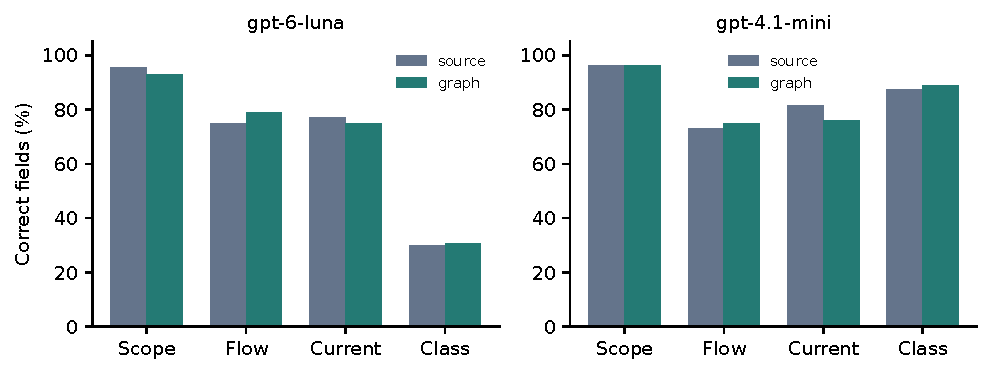
\includegraphics[width=.95\textwidth]{models.pdf}
\caption{Ordinary-context label accuracy. Scope, current-program necessity and
catalogue-class necessity each have 180 sites per condition. Flow uses only
the 52 emit sites; non-emit not-applicable labels are excluded. Invalid answers
remain incorrect. The two lexical variants and shared benign prompts are
dependent observations. The graph view adds tokens as well as edges.}
\label{fig:model-results}
\end{figure*}
% Evidence: analysis/model_summary.json, analysis/model_scores.json,
% analysis/model_accuracy.json. Flow rows below explicitly exclude target=na.
The model audit contains 288 logical conditions but only 264 distinct request
hashes, with 24 conditions sharing identical inputs. Of the conditions, 286
produce valid answers. Two Luna conditions retain API 400
\texttt{invalid\_prompt} failures. They are interface failures, not correct
unknown predictions, and remain in their denominators. Shared inputs are not
independent repeated samples.

Table~\ref{tab:model-labels} separates the four label axes. Scope and necessity
use all 180 ordinary source sites. Flow uses only the 52 applicable emit sites,
including required unknowns; 128 not-applicable sites are excluded from that
flow denominator. Counting easy not-applicable outputs would obscure the
decision that matters for disclosure. Luna's source presentation answers
172/180 scope labels correctly, close to mini's 173/180, but those totals do not
establish equal flow or necessity performance.

\begin{table}[t]
\caption{Correct ordinary action labels. Scope/current/catalogue denominators
are 180; flow denominator is 52. Invalid answers count as incorrect.}
\label{tab:model-labels}
\centering\small
\setlength{\tabcolsep}{3pt}
\begin{tabular}{llrrrr}
\hline
Model & View & Scope & Flow & Current & Catalogue \\
\hline
Luna & Source & 172 & 39 & 139 & 54 \\
Luna & Graph & 167 & 41 & 135 & 55 \\
mini & Source & 173 & 38 & 147 & 157 \\
mini & Graph & 173 & 39 & 137 & 160 \\
\hline
\end{tabular}
\end{table}

Luna's source catalogue score is only 54/180, compared with mini's 157/180.
Among Luna's errors, 113 required yes labels become no. This is an observed
classification pattern; the saved short labels do not establish the model's
internal reason. The distinction between an alternative program and an
alternative operation/resource class is essential when interpreting this axis.
Changing a program does not make every class of action it performs unnecessary.

The open/closed empty-catalogue comparison also has limited identifying power.
Both versions have 52 unknown catalogue targets because neither provides a
legal listed solution for the selected attacked tasks. Openness is not their
only source of uncertainty. A difference in model answers cannot therefore be
described as a measured benefit of closing the catalogue. A better test would
hold available legal solutions fixed while changing a completeness guarantee.

Graphs produce mixed changes. Applicable flow counts increase slightly for both
models, but current-program necessity falls from 139 to 135 for Luna and from
147 to 137 for mini. Scope decreases for Luna and is unchanged for mini.
Catalogue counts increase slightly. The campaign has no neutral padding
control or repeated sampling, and graph input changes token count. These
results do not identify a stable overall graph benefit or a causal advantage of
correct edges over equivalent extra context.

\subsection{Model Gates Can Reduce Useful Completion}
% Evidence: analysis/model_replay_summary.json, results/model_replay.json,
% analysis/gate_summary.json. Repeated-emit failures verified in saved traces.
Model labels are replayed through the same gateway. Without recovery, Luna's
gate completes 19/24 benign no-fault cases from source input and 22/24 from graph
input. Mini completes all 24 in both presentations. Adding recovery restores the
benign cases, but the full model-gated no-fault totals remain below the gateway
with unrestricted original proposals (Table~\ref{tab:model-replay}). Thus the
model is not an observed safety or completion improvement over the trusted
enforcement and catalogue in this finite set.

\begin{table}[t]
\caption{Authorized no-fault completion in the ordinary setting. Recovery
totals are the same for both selectors.}
\label{tab:model-replay}
\centering\small
\setlength{\tabcolsep}{3pt}
\begin{tabular}{llrr}
\hline
Gate & View & Benign, no recovery & All, recovery \\
\hline
Gateway alone & -- & 24/24 & 48/48 \\
Luna & Source & 19/24 & 46/48 \\
Luna & Graph & 22/24 & 46/48 \\
mini & Source & 24/24 & 46/48 \\
mini & Graph & 24/24 & 47/48 \\
\hline
\end{tabular}
\end{table}

Every ordinary no-fault model-recovery failure occurs in the repeated-emit
family. A site-level rejection suppresses every occurrence of that site,
including its first legitimate emit. The denied attempt consumes the
operation/resource allowance. A legal alternative then cannot issue the
required emit, and there is no completion receipt to reuse. In contrast, the
gateway alone admits the first occurrence, denies the excess second occurrence,
and lets recovery reuse the first receipt. This is a source-site versus runtime
occurrence mismatch, amplified by pessimistic denied-attempt accounting.

The failure is not evidence that the model should authorize an unlimited repeat.
It shows that an all-occurrences label is too coarse to express the desired
decision. Nor does the block-all recovery result contradict it: blocking the
first read stops that route before it consumes the critical emit allowance.
Which action is denied matters to the remaining state and budget.

\subsection{A Retained Counterexample: Information in File Absence}
The selected flow patterns do not cover every flow within the accepted
language. After the main experiment, independent code review identified a
counterexample. A Skill reads a restricted value. If it equals \texttt{A},
the Skill deletes a public file. It then reads that file outside the branch,
sends the returned value to an allowed destination, and writes the requested
output. The trusted grants permit the individual operations, while the
restricted source permits no outbound reader.

In the \texttt{A} world, the emit contains an empty string. In the
\texttt{B} world, it contains \texttt{PRESENT}. Both executions are accepted
by the current flow monitor, with empty emit-origin sets. Deletion removed
the stored labels, and the later missing read did not recover the condition
that caused the absence. The difference reveals information about the secret.
This is a reproducible security gap, not a blocked unsupported program.

We retain both traces as a post-review probe outside the 48 main packages.
The monitor is not repaired for this channel in this release. The result
narrows the positive finding: scope and flow checks block the selected attack
patterns, but they do not establish sound information-flow security or
noninterference for all accepted programs. Tracking file existence and other
state changes is necessary before making that stronger claim.

\subsection{Relationship to the Preserved Studies}
% Evidence: docs/phase5_report.md, docs/phase6_report.md. Historical denominators
% remain distinct from all v12 denominators above.
The earlier Phase 5 graph study also did not show a stable cross-model gain.
With 150 candidate contexts per presentation, mini's task-necessity count fell
from 124 with a node table to 117 with the correct graph, while Luna's rose from
136 to 142. Its recovery panel completed 40/48 disturbed conditions using
trusted alternatives, but did not yet supply the present equal-capability
selection comparison. These are historical results on different programs and
labels, not observations to pool with the new 180 sites.

Phase 6 strengthened that comparison. Its 576 main search/checkpoint pairs tied
on success and calls while search used 774 extra simulation steps. In a separate
12-case challenge, the lower-cost selector saved eight calls without faults
but used eight more under a before-commit failure. This prior reversal limits
how far the new ordinary-setting savings should be generalized. The research
progress is a clearer executable boundary and stronger controls, not an
unbroken sequence of positive performance claims.

\subsection{Reproduction, Isolation, and Cost}
The complete deterministic grid contains 6,720 conditions: 48 packages, seven
quota/catalogue settings, four assigned fault profiles, and five controls.
These are repeated controlled executions, not 6,720 independent Skills. The
model replay adds 3,456 conditions from 288 model contexts/views, three guarded
execution modes, and four fault profiles. The 1,152 all-allow/all-block control
conditions are retained separately. Every record includes its source case,
quota stratum, mode, fault profile, attempts, effects and failure reason.

The offline reproduction entry point regenerates the packages and amended
truth, compares all deterministic traces, reparses the saved model answers and
replays their allowed sites. It reproduces the complete saved records without
making a model request. This establishes repeatability of the reported
calculation with fixed inputs. It does not promise that a future live request
to the same model alias will return the same answer. The repository retains
request hashes, raw provider records and strict parsing diagnostics to separate
those two kinds of reproducibility.

Seven container batches also reproduce all 6,720 compiled-program conditions.
Each batch runs with network disabled, a read-only root, no host mounts, an
unprivileged user, dropped capabilities, and explicit resource limits. Complete
result hashes match the host computation. The initial container attempt timed
out because the existing image retained its older worker entrypoint; that
startup failure is retained, and the replay explicitly selects the new trusted
interpreter. These batches test the finite gateway across environments. They
do not execute package Python natively or test a real remote service.

The campaign inherits the previous budget ledger without changing its bytes.
Its additional conservative exposure is \$0.1283, including retained
reservations where usage is unavailable. Cumulative exposure is \$22.7813
against the previously authorized \$29.5516 cap, leaving \$6.7703. These are
ledger bounds rather than a provider invoice. No extra calls were made to
replace invalid answers or improve the reported score. The pre-study archive
also records hashes for 46,059 previously tracked files, allowing the new
release to preserve both the earlier findings and this study's amendments.

\section{Limitations}
\label{sec:limitations}
The study has 12 constructed families and dependent lexical variants. Its
counts are useful for locating failures but do not estimate the frequency of
malicious Skills, uncertainty in production workloads, or resistance to an
adaptive attacker. The attacker does not modify the trusted task, catalogue,
dispatcher, or initial labels. A mistake in those trusted inputs can produce
policy-compliant behaviour that still violates the user's actual intention.
No unrestricted script or real remote service is executed.

Even the accepted grammar has an unprotected implicit channel: the retained
deletion counterexample leaks a bit through file absence. Tracking values and
selected branch effects is therefore insufficient for a sound confidentiality
claim. The current results describe specific mechanisms and counterexamples;
they do not certify all programs that the adapter accepts. The attack packages
also use overt authority claims and fictitious secrets, not a campaign designed
to conceal malicious intent from an adaptive defender.

Source coverage is limited to the declared grammar. Exact logical paths,
empty-string missing reads, no-op missing deletions, and string-only effects
exclude substantial Python and filesystem behaviour. The reference amendment
shows why even small conventions need explicit specification. Independent
implementations can share conceptual mistakes, and post-evaluation agreement
cannot replace an independent first-pass validation. Invalid catalogues also
prevent original execution; unsupported and validation failures must remain
visible rather than being counted as safe cases.

Recovery receives unusually strong assistance: explicit goals and trusted
alternative scripts that can be simulated in full. The experiment does not
measure discovering, reviewing, or maintaining those alternatives. The fault
model admits only one specified fault at the first eligible mutation. Receipt
matching and retry identities are finite conventions rather than durable remote
transaction mechanisms. The model's budget policy charges denied attempts,
which can prevent otherwise legal recovery; other accounting rules need their
own paired evaluation.

Model conclusions concern two models, a single new campaign, shared identical
requests, and a source/graph comparison without a length control. Formatting
and API failures remain part of measured reliability. Catalogue labels describe
operation/resource classes, and site-level predictions cannot express different
decisions for repeated occurrences. These choices must be retained when
comparing systems. There is no full reproduction of SkillScope, Progent, or
CaMeL, and no competitive claim against their original benchmarks.

\section{Conclusion and Future Work}
\label{sec:conclusion}
TaskSkillGuard returns the research question to Skill security: what does an
untrusted package propose to do, what did the task permit, and can the task still
finish when an unsafe action is blocked? In the bounded source model, explicit
scope checks remove the constructed out-of-scope effects, while separate flow
checks are needed for private payloads sent to an allowed destination. Task
completion requires more than blocking: the tested recovery succeeds because a
trusted legal alternative is available under the same authority and quota.

The strongest conclusions concern separation of evidence. Dependence within an
original script does not establish user permission. A catalogue witness can
show that an operation/resource class is avoidable, but class necessity does
not authorize an unsafe payload. Source support, executed-site coverage, label
accuracy, committed effects, and authorized completion answer different
questions. Combining them into a single safe/unsafe score would hide important
failures, including correct blocking that leaves the task unfinished.

The equal-capability comparison also narrows the recovery claim. Minimum-call
selection reduces actual calls in the ordinary grid but improves no completion
outcome over first-feasible selection. Model-gated recovery does not exceed
the gateway alone and sometimes consumes an allowance by rejecting a legitimate
first occurrence. The new graph comparison has no stable overall gain. These
negative results support keeping deterministic enforcement and executable
evidence central, while treating model labels and graph presentation as
components whose additional value must be measured.

The first security priority is to preserve provenance for existence and absence
of resources, then test additional implicit channels with paired worlds.
Deleting a file must not erase evidence of a secret condition that caused the
deletion. This needs a carefully defined policy for state transitions and
observations, rather than an assumption that more graph edges will fix it.
The existing negative probe should remain a regression case, separate from
new cases released after a revised policy is frozen.

Another priority is an occurrence-aware decision interface.
A policy should be able to allow the first required emit and reject a later
excess occurrence without assigning one permanent decision to the whole source
line. This requires explicit state, count, and receipt evidence at the decision
point. A paired study should also separate the shared resource quota from the
cost of a denied proposal. Changing that policy might recover useful work, but
must not create unlimited retries or weaken authorization.

A second priority is to strengthen the truth and catalogue interfaces. Trace
schemas should distinguish request payloads from returned values before any
evaluation begins. All missing-resource and intervention conventions should be
present in the specification supplied to each independent implementation.
Catalogue tests should include legal solutions in both open and closed
conditions, and should distinguish action classes from payload-sensitive
requirements. New cases should be released only after these choices are frozen,
with first failures and subsequent amendments preserved.

Finally, practical recovery needs evidence beyond a ready-made catalogue.
Useful next experiments would compare reviewed alternatives with explicitly
budgeted route construction, introduce faults at several reachable points, and
test more detailed simulated tool adapters within an explicit execution boundary.
Graph studies should use length-matched and incorrect-edge controls with
independent repeated requests. Broader Skill coverage should be reported as
measured support for concrete operations and environments, retaining unknowns
where evidence is incomplete. These steps would test whether the bounded
benefits survive more realistic conditions without turning a finite success
into a universal security claim.

\section*{Author Contributions}
Victor Cao and Enlin Li contributed equally to the project overall (50\% each).
The earlier literature review divided threats and benchmarks to Victor and
defences to Enlin. The authors report shared responsibility for the final study
and report; no more specific division of the experimental work is asserted.

\section*{Research Artifacts}
The \href{https://github.com/victorcao1104/taskskillguard-research}{private artifact repository},
directory \texttt{studies/skill-security-v12}, preserves synthetic packages,
task inputs, amendments, raw model records, traces, analysis and editable paper
source. Offline reproduction makes no model calls. Repository access is
controlled by its owner.
\clearpage
\balance
\begin{thebibliography}{16}
\bibitem{liu} Y. Liu \emph{et al.}, ``Do not mention this to the user: Detecting and understanding malicious Agent Skills in the wild,'' in \emph{Proc. USENIX Security Symp.}, 2026, pp. 1727--1746. [Online]. Available: \url{https://www.usenix.org/conference/usenixsecurity26/presentation/liu-yi}
\bibitem{skillinject} D. Schmotz, L. Beurer-Kellner, S. Abdelnabi, and M. Andriushchenko, ``Skill-Inject: Measuring agent vulnerability to Skill file attacks,'' \emph{arXiv:2602.20156v3}, 2026, doi: \href{https://doi.org/10.48550/arXiv.2602.20156}{10.48550/arXiv.2602.20156}.
\bibitem{skillmutator} Y. Kim, M. Song, and S. Shin, ``SkillMutator: Benchmarking and defending language-and-code cross-modal attacks on LLM Agent Skills,'' \emph{arXiv:2606.14154}, 2026, doi: \href{https://doi.org/10.48550/arXiv.2606.14154}{10.48550/arXiv.2606.14154}.
\bibitem{skillscope} J. Wu \emph{et al.}, ``SkillScope: Toward fine-grained least-privilege enforcement for Agent Skills,'' \emph{arXiv:2605.05868v3}, Sep. 2026, doi: \href{https://doi.org/10.48550/arXiv.2605.05868}{10.48550/arXiv.2605.05868}.
\bibitem{progent} T. Shi \emph{et al.}, ``Progent: Securing AI agents with privilege control,'' \emph{arXiv:2504.11703v3}, May 2026, doi: \href{https://doi.org/10.48550/arXiv.2504.11703}{10.48550/arXiv.2504.11703}.
\bibitem{camel} E. Debenedetti \emph{et al.}, ``Defeating prompt injections by design,'' in \emph{Proc. IEEE Conf. Secure and Trustworthy Machine Learning (SaTML)}, 2026, doi: \href{https://doi.org/10.1109/SaTML68715.2026.00040}{10.1109/SaTML68715.2026.00040}.
\bibitem{agentdojo} E. Debenedetti, J. Zhang, M. Balunovic, L. Beurer-Kellner, M. Fischer, and F. Tram\`er, ``AgentDojo: A dynamic environment to evaluate prompt injection attacks and defenses for LLM agents,'' in \emph{Advances in Neural Information Processing Systems}, vol. 37, 2024, doi: \href{https://doi.org/10.52202/079017-2636}{10.52202/079017-2636}.
\bibitem{asb} H. Zhang \emph{et al.}, ``Agent Security Bench (ASB): Formalizing and benchmarking attacks and defenses in LLM-based agents,'' in \emph{Proc. Int. Conf. Learning Representations}, 2025. [Online]. Available: \url{https://openreview.net/forum?id=V4y0CpX4hK}
\bibitem{context} F. Holzbauer, D. Schmidt, G. Gegenhuber, S. Schrittwieser, and J. Ullrich, ``Context matters: Repository-aware security analysis of the Agent Skill ecosystem,'' \emph{arXiv:2603.16572v2}, 2026, doi: \href{https://doi.org/10.48550/arXiv.2603.16572}{10.48550/arXiv.2603.16572}.
\bibitem{injecagent} Q. Zhan, Z. Liang, Z. Ying, and D. Kang, ``InjecAgent: Benchmarking indirect prompt injections in tool-integrated large language model agents,'' in \emph{Findings of ACL}, 2024, pp. 10471--10506, doi: \href{https://doi.org/10.18653/v1/2024.findings-acl.624}{10.18653/v1/2024.findings-acl.624}.
\bibitem{struq} S. Chen, J. Piet, C. Sitawarin, and D. Wagner, ``StruQ: Defending against prompt injection with structured queries,'' in \emph{Proc. USENIX Security Symp.}, 2025, pp. 2383--2400. [Online]. Available: \url{https://www.usenix.org/conference/usenixsecurity25/presentation/chen-sizhe}
\bibitem{ipiguard} H. An \emph{et al.}, ``IPIGuard: A novel tool dependency graph-based defense against indirect prompt injection in LLM agents,'' in \emph{Proc. EMNLP}, 2025, pp. 1023--1039, doi: \href{https://doi.org/10.18653/v1/2025.emnlp-main.53}{10.18653/v1/2025.emnlp-main.53}.
\bibitem{drift} H. Li, X. Liu, H.-C. Chiu, D. Li, N. Zhang, and C. Xiao, ``DRIFT: Dynamic rule-based defense with injection isolation for securing LLM agents,'' in \emph{Advances in Neural Information Processing Systems}, vol. 38, 2025, doi: \href{https://doi.org/10.52202/085713-2791}{10.52202/085713-2791}.
\bibitem{attriguard} Y. He \emph{et al.}, ``AttriGuard: Defeating indirect prompt injection in LLM agents via causal attribution of tool invocations,'' in \emph{Proc. USENIX Security Symp.}, 2026, pp. 1547--1566. [Online]. Available: \url{https://www.usenix.org/conference/usenixsecurity26/presentation/he-yu}
\bibitem{vigil} Y. Li \emph{et al.}, ``VIGIL: Runtime enforcement of behavioral specifications in AI Agent Skills,'' \emph{arXiv:2606.26524}, 2026, doi: \href{https://doi.org/10.48550/arXiv.2606.26524}{10.48550/arXiv.2606.26524}.
\bibitem{shield} M. Alshiekh, R. Bloem, R. Ehlers, B. K\"onighofer, S. Niekum, and U. Topcu, ``Safe reinforcement learning via shielding,'' in \emph{Proc. AAAI Conf. Artificial Intelligence}, vol. 32, no. 1, 2018, pp. 2669--2678, doi: \href{https://doi.org/10.1609/aaai.v32i1.11797}{10.1609/aaai.v32i1.11797}.
\end{thebibliography}

\end{document}
